\documentclass[11pt,a4paper]{article}
%\documentclass{article}
\usepackage[utf8]{inputenc}
% 引入中文支持
%\usepackage{ctex}
\usepackage[top=2cm,bottom=1cm,left=2cm,right=2cm]{geometry}
\usepackage[BoldFont,SlantFont,CJKchecksingle]{xeCJK} %[BoldFont,SlantFont,CJKchecksingle]
\usepackage{ulem}
\usepackage{amsmath}
\usepackage{amsfonts}
\usepackage{amsthm}
\usepackage{amssymb}
\usepackage{array}
\usepackage{makecell}
\usepackage{fontspec}
\usepackage{xcolor}
\usepackage{titlesec}
\usepackage{setspace}
\usepackage{multirow}
\usepackage{indentfirst}
\usepackage{fancyhdr}
\usepackage{lastpage}
\usepackage{graphicx}
\usepackage{fontspec,xunicode}

\defaultfontfeatures{Mapping=tex-text}

\setlength{\headheight}{15pt}
\setlength{\parindent}{2em}

\setcounter{secnumdepth}{0} % 无标号

\newcommand\fontnameroman{Dustismo Roman}
\setCJKmainfont[BoldFont=SimHei]{SimSun}
\setCJKmonofont{simfang.ttf}
\setCJKsansfont{simhei.ttf}
\setCJKfamilyfont{fdsn}{FandolSong}
\newcommand{\stfdsn}{\CJKfamily{fdsn}}
\setCJKfamilyfont{song}{SimSun}                             %宋体 song
\newcommand{\song}{\CJKfamily{song}}
\setCJKfamilyfont{fs}{FangSong_GB2312}                      %仿宋2312 fs
\newcommand{\fs}{\CJKfamily{fs}}
\setCJKfamilyfont{yh}{Microsoft YaHei}                    %微软雅黑 yh
\newcommand{\yh}{\CJKfamily{yh}}
\setCJKfamilyfont{hei}{SimHei}                              %黑体  hei
\newcommand{\hei}{\CJKfamily{hei}}
\setCJKfamilyfont{hwxh}{STXihei}                                %华文细黑  hwxh
\newcommand{\hwxh}{\CJKfamily{hwxh}}
\setCJKfamilyfont{asong}{Adobe Song Std}                        %Adobe 宋体  asong
\newcommand{\asong}{\CJKfamily{asong}}
\setCJKfamilyfont{ahei}{Adobe Heiti Std}                            %Adobe 黑体  ahei
\newcommand{\ahei}{\CJKfamily{ahei}}
\setCJKfamilyfont{akai}{Adobe Kaiti Std}                            %Adobe 楷体  akai
\newcommand{\akai}{\CJKfamily{akai}}

\titleformat*{\section}{\LARGE\sffamily\bfseries}
\titleformat*{\subsection}{\Large\sffamily\bfseries}

\newtheorem{theorem}{Theorem}[section]
\newtheorem{lemma}[theorem]{Lemma}

\pagestyle{fancy}
\fancyhead{}
\fancyfoot[CO]{\sffamily page \thepage\ of \pageref{LastPage}} 
\fancyhead[CH]{SDWC Day4}
\fancyhead[RH]{\rightmark}
\renewcommand{\headrulewidth}{0.4pt} 
\renewcommand{\footrulewidth}{0.4pt} 
%\setlength{\headheight}{-5pt}
\setlength{\headsep}{5pt}
\titlespacing*{\section} {2pt}{2pt}{2pt}
\titlespacing*{\subsection} {1pt}{1pt}{1pt}
\titlespacing*{\subsubsection}{1pt}{1pt}{1pt}

\date{Feburary 10, 2022}
\begin{document}
\begin{spacing}{1.25}
	\title{SDWC Day4}
	\author{吴清月}
	\maketitle\par
	\begin{center}
		\centering
		\begin{tabular}{|p{3.6cm} | p{3.0cm}| p{3.0cm} | p{3.0cm}|}
			\hline
			\makecell[c]{\texttt{中文题目}} & \makecell[c]{\texttt{序列函数}} & \makecell[c]{\texttt{构树}} & \makecell[c]{\texttt{二分图}} \\
			\hline
			\makecell[c]{\texttt{英文题目}} & \makecell[c]{\texttt{Function}} & \makecell[c]{\texttt{Tree}} & \makecell[c]{\texttt{Tree}} \\
			\hline
			\makecell[c]{\texttt{程序名}} & \makecell[c]{\texttt{function.c/cpp}} & \makecell[c]{\texttt{tree.c/cpp}} & \makecell[c]{\texttt{graph.c/cpp}} \\
			\hline
			\makecell[c]{\texttt{输入文件}} & \makecell[c]{\texttt{function.in}} & \makecell[c]{\texttt{tree.in}} & \makecell[c]{\texttt{graph.in}} \\
			\hline
			\makecell[c]{\texttt{输出文件}} & \makecell[c]{\texttt{function.out}} & \makecell[c]{\texttt{tree.out}} & \makecell[c]{\texttt{graph.out}} \\
			\hline
			\makecell[c]{\texttt{每个测试点时限}} & \makecell[c]{\texttt{1.0 s}} & \makecell[c]{\texttt{1.0 s}} & \makecell[c]{\texttt{1.0 s}} \\
			\hline
			\makecell[c]{\texttt{测试点数目}} & \makecell[c]{\texttt{10}} & \makecell[c]{\texttt{10}} & \makecell[c]{\texttt{10}} \\
			\hline
			\makecell[c]{\texttt{每个测试点分值}} & \makecell[c]{\texttt{10}} & \makecell[c]{\texttt{10}} & \makecell[c]{\texttt{10}} \\
			\hline
			\makecell[c]{\texttt{附加样例文件}} & \makecell[c]{\texttt{有}} & \makecell[c]{\texttt{有}} & \makecell[c]{\texttt{有}} \\
			\hline
			\makecell[c]{\texttt{题目类型}} & \makecell[c]{\texttt{传统}} & \makecell[c]{\texttt{传统}} & \makecell[c]{\texttt{传统}} \\
			\hline
			\makecell[c]{\texttt{运行内存上限}} & \makecell[c]{\texttt{512M}} & \makecell[c]{\texttt{512M}} & \makecell[c]{\texttt{512M}} \\
			\hline
		\end{tabular}
	\end{center}\par
	\textbf{注意事项:} \par
	1. 无特别声明时, 结果比较方式为逐行比较模式(忽略多余空格和制表符).  \par
	2. C++语言源程序名称为题目名.cpp.  \par
	3. 编译命令为 \verb|g++ -o 题目名 题目名.* -lm -Wl,--stack=512000000 -O2 -std=c++11|. 即\textbf{评测时开启 O2 优化开关. 开启无限栈. 开启 C++11. 由于 11 特性导致的编译错误可以申请重测.} \par
	4. 文件名(程序名和输入输出文件名)必须使用英文小写.  \par
	5. 函数 \verb|main()| 的返回值类型必须是 \verb|int|, 程序正常结束时返回值必须是 \verb|0|.  \par
	6. 评测在Windows 11环境下用Lemon进行, 对于 \verb|long long| 类型使用 \verb|%lld|. 实际评测时限可能更改.  \par
	\thispagestyle{empty}
	\newpage
	\section{Problem A. 序列函数(function.c/cpp)} 
		\begin{tabbing}
			\hspace{4cm} \= \kill
			\indent  Input file: \> \texttt{function.in} \\
			\indent  Output file: \> \texttt{function.out} \\
			\indent  Time Limit : \> 1.0 second \\
			\indent  Memory Limit: \> 512 megabytes 
		\end{tabbing}

		有这么一个定义在序列上的函数 $f$,它的计算方法如下:

		$$f(a_1,a_2,\ldots,a_n)=\begin{cases}a_1&\text{if $n=1$}\\f(a_1\oplus a_2,a_2\oplus a_3,\ldots,a_{n-1}\oplus a_n)&\text{else}\end{cases}$$

		其中 $\oplus$ 表示按位异或。

		对于给定的数列 $a_1,a_2,\ldots,a_n$,你需要回答 $m$ 组询问,每次询问一个区间 $[l,r]$,你需要计算下面这个式子的结果:

		$$\max_{l\leqslant i\leqslant j\leqslant r} f(a_i,a_{i+1},\ldots,a_j)$$

		\subsection{Input}

		第一行两个整数 $n,m$。

		接下来一行 $n$ 个整数 $a_1,a_2,\ldots,a_n$。

		接下来 $m$ 行,每行两个整数 $l,r$ 表示一次询问。

		\subsection{Output}

		对于每次询问,输出一行一个整数,表示答案。

		\subsection{Examples}
			\begin{center}
				\centering
				\begin{tabular}{|p{7.2cm} | p{7.2cm}|}
					\hline
					\makecell[c]{\texttt{function-sample0.in}}&\makecell[c]{\texttt{function-sample0.ans}} \\
					\hline
					\makecell[tl]{
						\texttt{10 5}\\
						\texttt{1 2 3 4 5 6 7 8 9 10}\\
						\texttt{1 4}\\
						\texttt{2 9}\\
						\texttt{3 8}\\
						\texttt{5 6}\\
						\texttt{7 10}\\
					} &
					\makecell[tl]{
						\texttt{7}\\
						\texttt{15}\\
						\texttt{15}\\
						\texttt{6}\\
						\texttt{15}\\
					} \\
					\hline
				\end{tabular}
			\end{center}
		\subsection{Notes}

		数据规模与约定:

		对于 $30\%$ 的数据,保证 $n,m\leqslant 50$;

		对于 $50\%$ 的数据,保证 $n,m\leqslant 300$;

		对于 $100\%$ 的数据,保证 $1\leqslant n\leqslant 1000,0\leqslant m\leqslant 10^6,0\leqslant a_i\leqslant 2^{64}-1$。

	\newpage

	\section{Problem B. 构树(tree.c/cpp)} 
		\begin{tabbing}
			\hspace{4cm} \= \kill
			\indent  Input file: \> \texttt{tree.in} \\
			\indent  Output file: \> \texttt{tree.out} \\
			\indent  Time Limit : \> 1.0 seconds \\
			\indent  Memory Limit: \> 512 megabytes 
		\end{tabbing}\par
		有一天,你得到了一个 $n$ 个点的树。

		你感到很开心,于是记了下来和每一个点相邻的所有点中,编号最小的那个点和编号最大的那个点是什么。

		然而一段时间后,你把那棵树弄丢了,但是你记录的信息还保存着。

		你想得到原来的那棵树,于是尝试构造一个满足条件的解。

		\subsection{Input}

		第一行一个整数 $n$ ,表示树的点数。

		接下来 $n$ 行,每一行两个整数,表示和这个点相连的编号最小的点和编号最大的点。

		\subsection{Output}
		
		如果没有解,输出"-1"(不含双引号)。

		否则,输出 $n-1$ 行,每一行两个整数 $(a,b)$ ,描述一条边。

		如果有多种情况满足条件,你只需要输出任意一组合法解即可。

		\subsection{Examples}
			\begin{center}
				\centering
				\begin{tabular}{|p{7.2cm} | p{7.2cm}|}
					\hline
					\makecell[c]{\texttt{tree-sample0.in}}&\makecell[c]{\texttt{tree-sample0.ans}} \\
					\hline
					\makecell[tl]{
						\texttt{6}\\
						\texttt{5 5}\\
						\texttt{5 5}\\
						\texttt{4 4}\\
						\texttt{3 5}\\
						\texttt{1 6}\\
						\texttt{5 5}\\
					} &
					\makecell[tl]{
						\texttt{1 5}\\
						\texttt{2 5}\\
						\texttt{3 4}\\
						\texttt{4 5}\\
						\texttt{5 6}\\
					} \\
					\hline
				\end{tabular}
			\end{center}
			\begin{center}
				\centering
				\begin{tabular}{|p{7.2cm} | p{7.2cm}|}
					\hline
					\makecell[c]{\texttt{tree-sample1.in}}&\makecell[c]{\texttt{tree-sample1.ans}} \\
					\hline
					\makecell[tl]{
						\texttt{9}\\
						\texttt{5 5}\\
						\texttt{4 4}\\
						\texttt{6 6}\\
						\texttt{2 7}\\
						\texttt{1 9}\\
						\texttt{3 8}\\
						\texttt{4 4}\\
						\texttt{6 6}\\
						\texttt{5 5}\\
					} &
					\makecell[tl]{
						\texttt{1 5}\\
						\texttt{2 4}\\
						\texttt{3 6}\\
						\texttt{4 5}\\
						\texttt{4 6}\\
						\texttt{4 7}\\
						\texttt{5 9}\\
						\texttt{6 8}\\
					} \\
					\hline
				\end{tabular}
			\end{center}
			\begin{center}
				\centering
				\begin{tabular}{|p{7.2cm} | p{7.2cm}|}
					\hline
					\makecell[c]{\texttt{tree-sample2.in}}&\makecell[c]{\texttt{tree-sample2.ans}} \\
					\hline
					\makecell[tl]{
						\texttt{3}\\
						\texttt{2 3}\\
						\texttt{1 3}\\
						\texttt{1 2}\\
					} &
					\makecell[tl]{
						\texttt{-1}\\
					} \\
					\hline
				\end{tabular}
			\end{center}
		\subsection{Notes}

		数据规模与约定:

		对于 $10\%$ 的数据,保证 $1\le n\le 3$ ;

		对于 $30\%$ 的数据,保证 $1\le n\le 10$ ;
		
		对于另外 $20\%$ 的数据,保证存在一组解,使得树是一条链;
		
		对于 $100\%$ 的数据,保证 $1\le n\le 1000$ 。
		
	\newpage

	\section{Problem C. 二分图(graph.c/cpp)} 
		\begin{tabbing}
			\hspace{4cm} \= \kill
			\indent  Input file: \> \texttt{graph.in} \\
			\indent  Output file: \> \texttt{graph.out} \\
			\indent  Time Limit : \> 1.0 seconds \\
			\indent  Memory Limit: \> 512 megabytes 
		\end{tabbing}\par
		从前有一张 $n$ 个点,$m$ 条边的二分图。

		你觉得这张图太过稀疏了,于是想往这张图里添加一些边。

		为了方便自己写匹配算法,你希望在添加完边之后,图仍然是二分图。

		求最多能够添加多少条边。

		\subsection{Input}

		第一行两个整数 $n,m$,表示图的点数和边数。

		接下来 $m$ 行,每行两个整数 $u,v$,描述一条边。

		保证给出的是二分图。

		\subsection{Output}

		输出一行一个整数,表示最多还能添加多少条边。

		\subsection{Examples}
			\begin{center}
				\centering
				\begin{tabular}{|p{7.2cm} | p{7.2cm}|}
					\hline
					\makecell[c]{\texttt{graph-sample0.in}}&\makecell[c]{\texttt{graph-sample0.ans}} \\
					\hline
					\makecell[tl]{
						\texttt{4 2}\\
						\texttt{1 2}\\
						\texttt{3 4}\\
					} &
					\makecell[tl]{
						\texttt{2}\\
					} \\
					\hline
				\end{tabular}
			\end{center}
			样例解释:

			一种可能的解如下:

			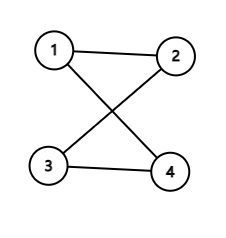
\includegraphics{pic/1.png}
		\subsection{Notes}

		数据规模与约定:

		对于 $20\%$ 的数据,保证 $n\leq 10$;

		对于另外 $20\%$ 的数据,保证给出的图连通且为一棵树;

		对于另外 $10\%$ 的数据,保证 $m=0$;

		对于另外 $20\%$ 的数据,保证连通块数量 $\leqslant 3$;

		对于 $100\%$ 的数据,保证 $\displaystyle 1\leq n\leq 5000,0\leqslant m\leqslant \frac{n(n-1)}{2}$。
	\newpage
		
\end{spacing}
\end{document}
